% !TeX program = lualatex
% !TeX encoding = utf8
% !BIB program = biber

\documentclass{bachelor_report}

% Додаткові пакети вносіть у цей файл
%%%% У даний файл додавайте всі необхідні вам додаткові пакети, наприклад...

\usepackage[h]{esvect} % fancy vector arrows

\usepackage[bibstyle=gost-numeric,sorting=none]{biblatex}
\addbibresource{bach_report.bib}
\usepackage[autostyle=false]{csquotes}
\renewcommand{\bibfont}{}

\usepackage{fontspec}
\setmainfont{CMU serif}

\usepackage{microtype}

\usepackage{bbm} % for using indicator \mathbbm{1}

\usepackage{tikz}
\usepackage{pgfplots}
\pgfplotsset{compat=1.3}

\usepackage{tabularray} % пакет для просунутих таблиць

\usepackage{xcolor}
% \pagecolor[rgb]{0.118,0.118,0.118}
% \color[rgb]{0.8,0.8,0.8}

% Додаткові визначення та перевизначення команд вносіть у цей файл
%%% У даному файлі визначайте всі необхідні вам нові команди TeX
%%% або робіть перевизначення існуючих, наприклад...

% Перевизначення символу порожньої множини та знаків "більше-дорівнює", "менше-дорівнює" на прийняті у нас
\let\oldemptyset\emptyset
\let\emptyset\varnothing
\let\geq\geqslant
\let\leq\leqslant

% Визначення нових математичних команд
\newcommand*{\binsp}[1]{\ensuremath \left\{0, 1\right\}^{#1}}       % {0, 1}^m
\newcommand*{\xor}{\ensuremath \oplus}                              % \xor = (+)
\newcommand*{\GF}[1]{\ensuremath \mathbb F_{#1}}                    % F_n
\newcommand*{\GFgroup}[1]{\ensuremath \mathbb F^{*}_{#1}}           % F^*_n
\newcommand*{\Zring}[1]{\ensuremath \mathbb Z_{#1}}                 % Z_n
\newcommand*{\Zgroup}[1]{\ensuremath \mathbb Z^{*}_{#1}}            % Z^*_n
\newcommand*{\Jset}[1]{\ensuremath \mathbb J_{#1}}                  % J_n
\newcommand*{\Qset}[1]{\ensuremath \mathbb Q_{#1}}                  % Q_n
\newcommand*{\PQset}[1]{\ensuremath \widetilde{\mathbb Q}_{#1}}     % Q~_n
\newcommand*{\cyclic}[1]{\ensuremath \left\langle {#1} \right\rangle}                  % <g>
\newcommand*{\Legendre}[2]{\ensuremath \left( \frac{#1}{#2} \right)}  % символ Лежандра/Якоби
\newcommand*{\compinv}[1]{\ensuremath {#1}^{\left\langle -1 \right\rangle}}  % обратный по композиции

% Інший спосіб визначення математичного оператору
\DeclareMathOperator{\ord}{ord}
\DeclareMathOperator{\lcm}{lcm}
\DeclareMathOperator{\Li}{Li}
\DeclareMathOperator{\Coef}{Coef}
\DeclareMathOperator{\Log}{Log}
\DeclareMathOperator{\Exp}{Exp}
\DeclareMathOperator{\Res}{Res}
\DeclareMathOperator{\charact}{char}
\DeclareMathOperator{\Sym}{Sym}


% команда для коментарів червоним кольором
% !!! Конфлікт пакету color з якимось іншим пакетом, не використовувати
%\newcommand{\todo}[1]{\textcolor{red}{#1}}


%%% ...і таке інше

% Відомості про автора роботи
%%% Основные сведения %%%
\newcommand{\reportAuthor}             % ФИО автора
{ПІБ автора}
\newcommand{\reportAuthorGroup}        % группа автора
{ФХ-N3}
\newcommand{\reportTitle}              % Название (тема исследования)
{Назва дослідження}
%% використовуйте символ "\par" або "\\" для розбиття назви на декілька рядків


\newcommand{\supervisorFio}            % Научный руководитель, ФИО
{Прізвище І.П.}
\newcommand{\supervisorRegalia}        % Научный руководитель, регалии
{степінь, звання}

% Починаємо верстку документа
\begin{document}

\setfontsize{14}

% Створюємо титульну сторінку
% Титульный лист
\thispagestyle{empty}

\begin{center}
НАЦІОНАЛЬНИЙ ТЕХНІЧНИЙ УНІВЕРСИТЕТ УКРАЇНИ \par
<<КИЇВСЬКИЙ ПОЛІТЕХНІЧНИЙ ІНСТИТУТ ім. Ігоря СІКОРСЬКОГО>>\par
НАВЧАЛЬНО-НАУКОВИЙ ФІЗИКО-ТЕХНІЧНИЙ ІНСТИТУТ\par

\vspace{40mm}
{\huge Звіт з виконання кваліфікаційного дослідження \par}

\huge\MakeUppercase{\textbf{\reportTitle}} \par
\end{center}

\vspace{40mm}
\begin{flushright}
Виконав студент

групи \reportAuthorGroup

\reportAuthor

\vspace{20mm}
Науковий керівник:

\supervisorRegalia

\supervisorFio

\end{flushright}

\vspace{20mm}
\begin{center}
{Київ~--- 2022}
\end{center}

\newpage
\thispagestyle{plain}


%% Створюємо зміст    % -- розкоментуйте, якщо зміст вам потрібен
%\pagenumbering{gobble}
%\tableofcontents
%\cleardoublepage
%\pagenumbering{arabic}

\setcounter{page}{2}    %!!! -- продумати, як автоматизувати номер сторінки

%% Якщо ви використовуєте зміст, то прослідкуйте, щоб номер сторінки 
%% співпадав із справжнім!

% Створюємо перелік умовних позначень, скорочень і термінів
% Якщо цей розділ вам не потрібен, просто закоментуйте два наступних рядка
\shortings
%!TEX root = ../thesis.tex
% створюємо перелік умовних позначень, скорочень і термінів
ФТІ --- Фізико-технічний інститут

$\xor$ --- операція побітового додавання  %зауважте, що використовується перевизначена операція \xor


(Якщо ви не використовуєте перелік умовних позначень, просто приберіть 
даний розділ.)

(БУДЬ ЛАСКА, ПРОСЛІДКУЙТЕ, ЩОБ НОМЕР СТОРІНКИ СПІВПАДАВ ІЗ СПРАВЖНІМ! Це залежить від того, наскільки великим є ваш зміст.
Номер сторінки проставляється у файлі thesis.tex, рядок 35.)

% Створюємо вступ
\intro
%!TEX root = ../thesis.tex
% створюємо вступ
\textbf{Актуальність дослідження.} Актуальність даного дослідження полягає 
у тому, що без нього ви не одержите диплом про вищу освіту. Відповідно, ви повинні 
оформити результати вашого дослідження належним чином.

Вступ є однією із самих формалізованих частин дипломної роботи. На початку 
ви у двох-трьох абзацах повинні окреслити проблематику та актуальність 
вашого дослідження, після чого переходити до мети та завдання.

\textbf{Метою дослідження} є певна абстрактна недосяжна річ на кшталт 
загальнолюдського щастя на горизонті. Для досягнення мети необхідно 
розв'язати \textbf{задачу дослідження}, яка полягає у чомусь суттєво більш 
конкретному. Для розв'язання задачі необхідно вирішити такі завдання:

\begin{enumerate}
\item провести огляд опублікованих джерел за тематикою дослідження;
\item (наступний пункт, пов'язаний із теоретичним дослідженням);
\item (і ще один, наприклад, про експериментальну перевірку результатів);
\item (і взагалі, краще із науковим керівником проконсультуйтесь, як ваші 
завдання правильно писати).
\end{enumerate}

\emph{Об'єктом дослідження} є якісь процеси або явища загального 
характеру (наприклад, <<інформаційні процеси в системах криптографічного 
захисту>>).

\emph{Предметом дослідження} є конкретний математичний чи фізичний 
об'єкт, який розглядається у вашій роботі та який можна трактувати
як певну властивість об'єкта дослідження (наприклад, <<моделі та методи
диференціального криптоаналізу ітеративних симетричних блочних шифрів>>).

При розв’язанні поставлених завдань використовувались такі \emph{методи дослідження}: і 
тут коротенький перелік (наприклад, але не обмежуючись: методи лінійної та абстрактної 
алгебри, теорії імовірностей, математичної статистики, комбінаторного 
аналізу, теорії кодування, теорії складності алгоритмів, методи 
комп’ютерного та статистичного моделювання) 

\textbf{Наукова новизна} отриманих результатів полягає... -- тут необхідно 
перелічити, що саме нового з точки зору науки несе ваша робота. До усіх 
тверджень, які сюди виносяться, подумки (а іноді й явним чином) потрібно 
ставити слово <<вперше>> -- і ці твердження повинні залишатись істинними.

\textbf{Практичне значення} результатів полягає... -- тут необхідно 
зазначити практичну користь від результатів вашої роботи. Що саме можна 
покращити, підвищити (або знизити), зробити гарного (або уникнути 
поганого) після вашого дослідження.

\textbf{Апробація результатів та публікації.} Наприкінці вступу необхідно 
зазначити перелік конференцій, семінарів та публікацій, в яких викладено 
результати вашої роботи. Якщо результати вашої роботи ніде не 
доповідались, опускайте даний абзац.

% Додаємо глави
% Якщо ваша робота містить менше або більше глав - модифікуйте наступні 
% рядки відповідним чином
%!TEX root = ../thesis.tex

\chapter{(Назва першого розділу)}
\label{chap:review}  %% відмічайте кожен розділ певною міткою -- на неї наприкінці необхідно посилатись

На початку кожного розділу рекомендується вставити одне-два-абзац речень, 
у яких коротенько представили, про що тут взагалі буде мова.

\section{(Назва першого підрозділу)}

Перший розділ повинен бути присвячений огляду попередніх результатів за 
тематикою вашого дослідження. У даному розділі повинні міститись вс' 
визначення та описи, необхідні для подальшого викладення матеріалу, та результати 
ваших попередників.

Зауважимо, що наводити детальні доведення не ваших результатів необхідно 
наводити лише тоді, коли вони містять якусь вкрай важливу інформацію для 
саме ваших результатів.

Також зауважимо, що абсолютно на всі не ваші результати повинні стояти 
належним чином оформлені посилання.

Розмір першого (оглядового) розділу не повинен перевищувати третини вашої 
дипломної роботи (без урахування додатків).


\section{(Назва другого підрозділу)}

Наведемо основні правила оформлення текстів у системі \LaTeX.

Для абзацу робіть пусті рядки у файлі. Курсивний текст робиться командою 
emph: \emph{ось так}. Жирний текст робиться командою textbf: \textbf{ось так}.

<<Лапки>> робляться двома знаками більше та двома знаками менше. Довге 
тире у тексті --- трьома дефісами, коротке -- двома дефісами; у формулах 
мінуси робляться одним дефісом: $a-b$.

Пишіть звичайний текст звичайним текстом, а формули, позначення змінних та 
операцій (усі формули, усі позначення змінних та усі операції) беріть у 
знаки долара, ось так: $E = mc^2$, $a_1 = a^{(2)} \cdot a_{n, k}$, $e^x = 
\sum_{k = 0}^{\infty} {\frac{x^k}{k!}}$. Якщо вам 
не подобається, як \LaTeX подав формулу для експоненти (мені, наприклад, 
не подобається), то можна внести у код формули деякі корективи та написати ось так: $e^x 
= \sum\limits_{k = 0}^{\infty} {\dfrac{x^k}{k!}}$.

Для прикладу різні варіації коми у формулах: $(a, b)$ vs. $(a,b)$. Поки 
пакет icomma працює, різниця видна наочно.

Виключна формула (формула окремим рядком) робиться через подвійні знаки 
долара або через оточення equation. Зауважте, що при цьому змінюється 
оформлення формул:
$$e^x = \sum_{k = 0}^{\infty} {\frac{x^k}{k!}}.$$

Формули за помовчанням не підтримують кирилічні літери. Зверніть увагу на 
порожній рядок перед попереднім реченням у tex-файлі: без нього не буде 
створено абзац.

Із більш специфічних позначень --- ось так, скажімо, можна подати 
перестановку:
$$\pi = \begin{pmatrix}
1 & 2 & 3 & 4 & 5 & 6 & 7 & 8 & 9\\
a & 5 & 9 & 6 & 4 & 8 & 2 & 1 & 7
\end{pmatrix},$$
де $a=3$. Зауважте, що у попередньому реченні нема порожнього рядочку 
перед <<де>> (та, відповідно, абзацу після формули), а кома внесена у 
виключну формулу, бо інакше вона переїде у наступний рядок тексту.

Декілька формул поспіль треба збирати в єдине ціле оточеннями gather або 
eqnarray; назви оточень із зірочками вказують \LaTeX'у не нумерувати дані 
формули. Наприклад, ось рекуренти для циклових чисел та чисел Стірлінга 
I~роду:
\begin{eqnarray*}
c(n+1, k) &=& c(n, k-1)+nc(n, k); \\
s(n+1, k) &=& s(n, k-1)-ns(n, k).
\end{eqnarray*}

Зверніть увагу на символ <<\verb|~|>> у попередньому абзаці tex-файлу між 
<<I>> та <<роду>>; це нерозривний пробіл, який не дасть рознести пов'язані 
частини по різних рядках. Тільду треба ставити перед усіма посиланнями 
(команди ref та cite), перед тире та у місцях, які не можна розривати за 
правилами граматики.

Для специфічних позначень ви можете задавати власні команди (їх 
рекомендовано заносити у файл <<\verb|02_redefinitions|>>). Наприклад, 
подивіться, як оформлюється теорема Лагранжа-Бюрмана із використанням 
введених команд \verb|\Coef| та \verb|\compinv|:

\begin{theorem}[Лагранж, Бюрман] \label{thLagrangeBurmann}
Для будь-якого ряду $A \in x \mathcal R[[x]]_1$ та $k \in \mathbb N$ справедливе співвідношення
$$n \Coef[x^n] \left( \compinv{A}(x) \right)^k = k \Coef[x^{n-k}] \left(\! \frac{x}{A(x)} \!\right)^n.$$
\end{theorem}
\begin{proof}
Доведення ви подивитесь деінде, а тут подивіться, як воно оформлюється 
(зокрема, на квадратик наприкінці :)).                                                                                       
\end{proof}

\begin{corollary} \par %\label{pr##}
Будь-ласка, перевіряйте граматику. Латеховські редактори зазвичай не мають 
інтегрованих спелчекерів української мови, тому використовуйте сервіси, 
наведені, наприклад, тут: https://coma.in.ua/30584
\end{corollary}

Іноді написаний файл треба компілювати двічі для одержання ефекту 
(скажімо, для коректної побудови усіх гіперпосилань та побудови змісту). 
Скажімо, оце посилання на теорему~\ref{thLagrangeBurmann} (теорему 
Лагранжа-Бюрмана) з першої компіляції може показати вам знаки питання 
<<??>>. Однак після повторної компіляції ви одержите те, що потрібно.

Онлайн-сервіси на кшталт Overleaf справляються з такими ситуаціями за одну компіляцію. Однак той 
же Overleaf має звичку компілювати pdf-файли навіть за наявності помилок у 
тексті, просто ігноруючи відповідні місця. Якщо ви працюєте у Overleaf, 
то переконайтесь, що у вас нема червоних помилок після компіляції. На 
щастя, останні апдейти Overleaf вивалюють червоні помилки прямо вам в очі, 
тому їх нескладно помітити.

Якщо вам потрібна якась фіча, запитайте в Сенсея. Майже напевно вона є.

На жаль деякі пакети шаблону викликають незрозумілі конфлікти. Поки що не 
вдалось інтегрувати у шаблон такі пакети, як color та tikz. Якщо без 
кольорового забарвлення тексту ще можна пережити, то використовувати 
діаграми tikz поки що рекомендується за допомогою милиць:

\begin{itemize}
\item створюєте окремий допоміжний tex-проект, у якому за допомогою tikz створюєте 
діаграму;
\item компілюєте допоміжний tex-проект;
\item вставляєте створену діаграму з pdf-файлу у диплом як зображення.
\end{itemize}

Ми ж зі свого боку продовжуємо працювати над покращенням даного шаблону.

\section{(Назва третього підрозділу)}


Надамо деякі рекомендації щодо використання даного стильового файлу.

\begin{theorem}
Використовуйте оточення \emph{theorem} для теорем.
\end{theorem}
\begin{proof}
Для доведень використовуйте оточення \emph{proof}.
\end{proof}
\begin{theorem}
Нумерація відбувається автоматично
\end{theorem}
\begin{claim}
Використовуйте оточення \emph{claim} для тверджень.
\end{claim}
\begin{lemma}
Використовуйте оточення \emph{lemma} для лем.
\end{lemma}
\begin{corollary}
Використовуйте оточення \emph{corollary} для наслідків.
\end{corollary}
\begin{definition}
Використовуйте оточення \emph{definition} для визначень.
\end{definition}
\begin{example}
Використовуйте оточення \emph{example} для прикладів, на які є посилання.
\end{example}
\begin{remark}
Використовуйте оточення \emph{remark} для зауважень. Зверніть увагу, як 
веде себе команда \textbf{emph}
\end{remark}


\chapconclude{\ref{chap:review}}

Наприкінці кожного розділу ви повинні навести коротенькі підсумки по його 
результатах. Зокрема, для оглядового розділу в якості висновків необхідно 
зазначити, які задачі у даній тематиці вже були розв'язані, а саме 
поставлена вами задача розв'язана не була (або розв'язана погано), тому у 
наступних розділах ви її й розв'язуєте.

Якщо ваш звіт складається з одного розділу, пропускайте висновок до 
нього~-- він повністю включається в загальні висновки до роботи
%!TEX root = ../thesis.tex
% створюємо розділ
\chapter{(Назва другого розділу)}
\label{chap:theory}

До другого розділу також краще написати малесенький вступ. Зокрема, це 
збільшує загальний об'єм роботи та покращує її читабельність.

\section{(Якийсь підрозділ)}

У другому розділі необхідно наводити розв'язання поставленої перед вами 
задачі у теоретичному або аналітичному сенсі (хоча, звісно, все залежить 
від того, яка саме задача перед вами поставлена).

Для подання матеріалів можна використовувати таблиці (наприклад, 
Таблицю \ref{tab_weight}). Розмір шрифту у таблиці може бути меншим за 14~pt (наприклад, 12~pt, або навіть 10~pt, якщо так таблиця виглядає зрозуміліше та компактніше).

    \begin{table}[ht]
    \setfontsize{14pt}
    \caption{Розрахунок якоїсь фантастичної дичини у декілька кроків}
    \label{tab_weight}
    \centering
        \begin{tabular}{|c|c|c|c|c|c|c|c|c|}
        \hline \multirow{2}{*}{Параметр $x_i$} & \multicolumn{4}{c|}{Параметр $x_j$} & 
            \multicolumn{2}{c|}{Перший крок} & \multicolumn{2}{c|}{Другий крок} \\
        \cline{2-9} & $X_1$ & $X_2$ & $X_3$ & $X_4$ & $w_i$ & 
            ${K_\text{в}}_i$ & $w_i$ & ${K_\text{в}}_i$ \\
        \hline $X_1$ & 1 & 1 & 1.5 & 1.5 & 5 & 0.31 & 19 & 0.32 \\
        \hline $X_2$ & 1 & 1 & 1.5 & 1.5 & 5 & 0.31 & 19 & 0.32 \\
        \hline $X_3$ & 0.5 & 0.5 & 1 & 0.5 & 2.5 & 0.16 & 9.25 & 0.16 \\
        \hline $X_4$ & 0.5 & 0.5 & 1.5 & 1 & 3.5 & 0.22 & 12.25 & 0.20 \\
        \hline \multicolumn{5}{|c|}{Разом:} & 16 & 1 & 59.5 & 1 \\
        \hline
        \end{tabular}
    \end{table}

Бажано, щоб кожен пункт завдань, окреслених у вступі, відповідав певному 
розділу або підрозділу у дипломній роботі.

\begin{theorem}
Нумерація у наступних розділах також проставляється автоматично та коректно.
\end{theorem}

\section{(Якийсь наступний підрозділ з дуже-дуже довгою назвою, загальна кількість слів в якій, однак, не повинна перевищувати 12 слів)}

Для подання матеріалів також дуже зручними є рисунки (наприклад, рисунки 
\ref{fig_sudak} або \ref{fig_pacman}).


\begin{figure}[ht]
\centering
    \begin{subfigure}[b]{0.5\textwidth}    
        
\includegraphics[scale=0.3]{Images/Sudak.png}
        \caption{}
        % обратите внимание на знак % после \end{subfigure} и 
        % отсутствие пустых строк и разделителей после \end{subfigure}
        % -- это сливает в одну строку подфигуры
    \end{subfigure}%
    \begin{subfigure}[b]{0.5\textwidth}
        
\includegraphics[scale=0.3]{Images/Tudak.png}
        \caption{}
    \end{subfigure}
 
    \caption{Різні види риб: (a) судак, (б) тудак.}
    \label{fig_sudak}
\end{figure}

\begin{figure}[ht]
        \centering
        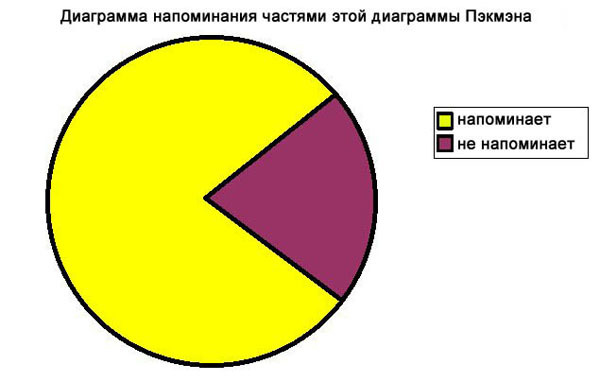
\includegraphics[scale=0.5]{Images/Pacman.jpg}
        \caption{Частка кругових діаграм, які схожі на Пекмена}
        \label{fig_pacman}
\end{figure}

\chapconclude{\ref{chap:theory}}

Наприкінці розділу знову наводяться коротенькі підсумки.

% Створюємо висновки
\conclusions
%!TEX root = ../thesis.tex
% створюємо Висновки до всієї роботи
Загальні висновки до роботи повинні підсумовувати усі ваші досягнення у 
даному напрямку досліджень.

За кожним пунктом завдань, поставлених у вступі, у висновках повинен 
міститись звіт про виконання: виконано, не виконано, виконано частково (І 
чому саме так). Наприклад, якщо першим поставленим завданням у вас іде 
<<огляд літератури за тематикою досліджень>>, то на початку висновків ви 
повинні зазначити, що <<у ході даної роботи був проведений аналіз 
опублікованих джерел за тематикою (...), який показав, що (...)>>. Окрім 
простої констатації про виконання ви повинні навести, які саме результати 
ви одержали та проінтерпретувати їх з точки зору поставленої задачі, мети 
та загальної проблематики.

В ідеалі загальні висновки повинні збиратись з висновків до кожного 
розділу, але ідеал недосяжний. :) Однак висновки не повинні містити 
формул, таблиць та рисунків. Дозволяється (та навіть вітається) 
використовувати числа (на кшталт <<розроблена методика дозволяє підвищити 
ефективність пустопорожньої балаканини на $2.71\%$>>).

Наприкінці висновків необхідно зазначити напрямки подальших досліджень: 
куди саме, як вам вважається, необхідно прямувати наступним дослідникам у 
даній тематиці.


% Додаємо бібліографію
% Якщо ви володієте магією bibtex-у, використовуйте її та модифікуйте файл 
% з бібліографією відповідним чином
%!TEX root = ../thesis.tex
% створюємо список використаної літератури
\begin{thebibliography}    
    \bibitem{sad} 
    asda

    \bibitem{dca}
    asd [Електронний ресурс]. --- Режим доступу: \url{dsf}.

 
\end{thebibliography}


% Створюємо додатки (дивись у файли додатків для необхідних пояснень)
% Якщо ви маєте меншу або більшу кількість додатків, модифікуйте наступні 
% рядки відповідним чином
% Якщо ви не маєте додатків, просто закоментуйте наступні рядки
%!TEX root = ../thesis.tex
\append{Тексти програм}
\label{appendix:A}

Тексти інструментальних програм для проведення експериментальних досліджень необхідно 
виносити у додатки.

\section{Програма 1}

Зауважте, як змінилась нумерація.
%!TEX root = ../thesis.tex
\append{Великі рисунки та таблиці}
\label{appendix:B}

Якщо результати вашої роботи описуються величезними рисунками і таблицями 
(один аркуш та більше) у незліченній кількості, іх також необхідно 
виносити у додатки.

% (Зробити ще два додатки -- приклади відгуку та рецензії)


% Нарешті
\end{document}